\section{Cognitive Architectures}
\label{sec:cogarch}
Cognitive architectures are architectures that base themselves on some model of human cognition. There are several competing theories about how cognition works, and one of the most well-supported is the Global Workspace Theory.

There hasn't been widespread research done with cognitive architectures, however. Arrabales et al put forth that this is perhaps because of poor understanding of cognitive research amongst researchers in the field of classical AI. \cite{arrabales2009gamechars}

There is many different cognitive architectures available today\cite{duch2008cognitive}. We chose to focus on those based on the Global Workspace theory, for several reasons. It's widely accepted as the currently best model of understanding consciousness\cite{Franklin2012}, implementations using it generally provide believable results\cite{arrabales2009gamechars}\cite{snaider2011lida} and it has a solid grounding in neurological and psychological models, experiments and empirical evidence\cite{Franklin2012}.

\subsection{Global Workspace Theory}
\begin{figure}[h!tb]
\centering
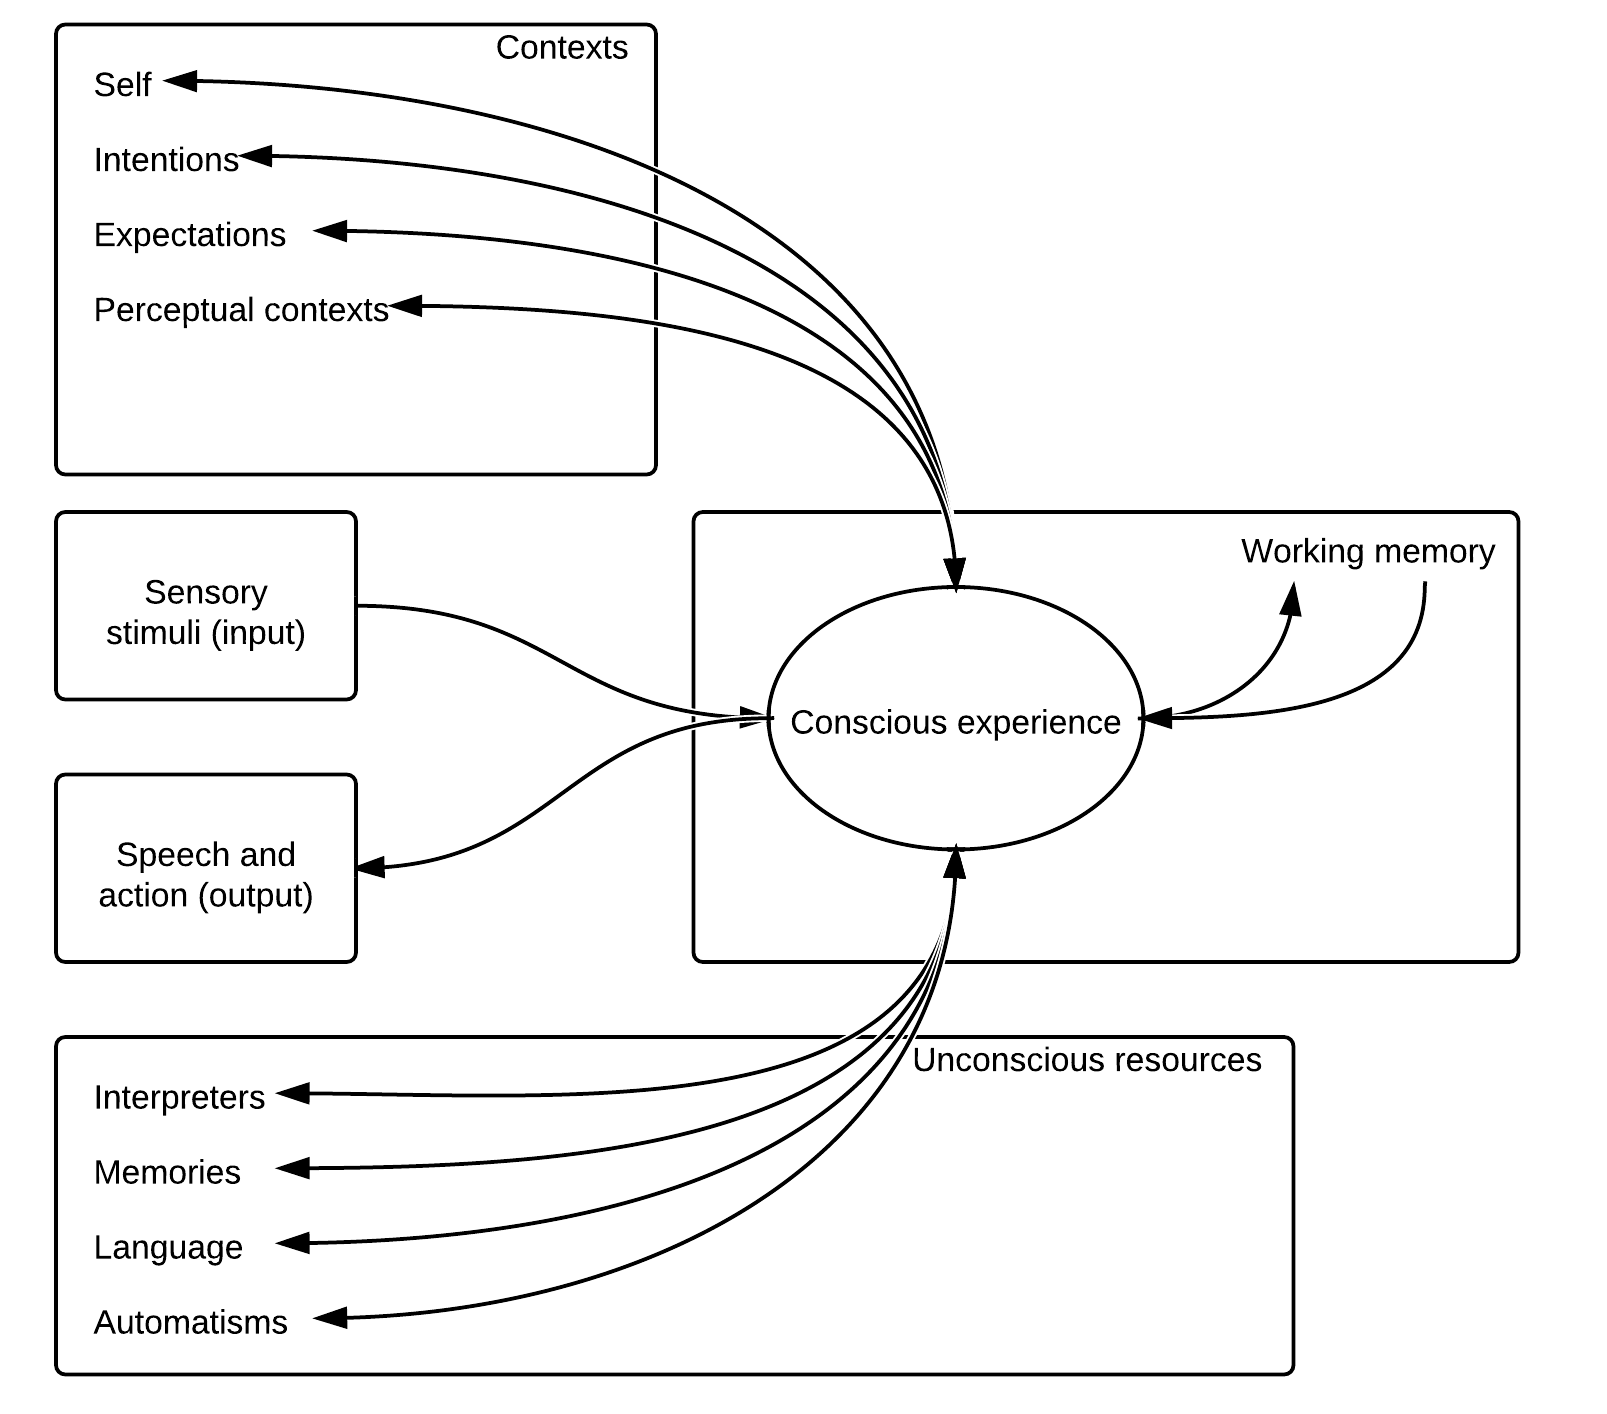
\includegraphics[scale=1.0]{graphics/globalworkspace.png}
\caption{A schematic of the Global Workspace theory\cite{baars2005gwt}}
\label{fig:gwt}
\end{figure}

Global Workspace Theory is a model of cognition that is very well supported by experimental data, and is one of the most widely accepted models. \cite{dehaene2001towards} It has been used to implement processes that imitate human decision making (for example for solving the problem of assigning people to jobs in the US Navy).\cite{baars2005gwt}\cite{franklin2003interacting}

It is based around an understanding of the brain as a set of many independently processing modules, working together by utilizing a shared workspace (hence the ``global workspace''). Every ``cognitive cycle'' all the processes compete for attention, and a single one gets the proverbial spotlight shone upon it.\cite{baars2005gwt} When this happens, all the other modules/processes receive the ``broadcasted'' data from that module, and use it as they see fit; for example memory centers store the information received. This solves the relevancy problem\footnote{The relevancy problem is part of the frame problem, the problem of knowing what to apply where in problem solving, and was considered to might be intractable.\cite{shanahan2005applying}}, and it lets parts of the brain collaborate on problems that can't be solved unconsciously by individual modules.

See figure \ref{fig:gwt} for a graphical overview of the theory.

\subsubsection{The theatre metaphor}
A common metaphor used is the {\em theatre metaphor}. Here we view the mind as a proverbial theatre, with an audience and a stage with a spotlight shining on it.

Then various actors on stage get the spotlight shone upon them (according to the pandemonium theory which is often used; the one who shouts the loudest\cite{selfridge1958pandemonium}), and is allowed to share its message with the the audience.

In the dark, behind the stage, are the various executive processes (represented by script writers, directors, etc.) who aren't visible but still help form what is seen.

\subsubsection{Neurological basis for the Global Workspace Theory}
According to R. Llinás et al.\cite{llinas1998neuronal}, the looped neural pathways between the thalamus and the cortex might be what is responsible for the conscious collaboration between various parts of the brain. The thalamus is responsible for letting various parts of the cortex broadcast and influence the rest of the cortex. This meshes well with the global workspace theory, and the idea of a single subsystem broadcasting its contents to the rest of the whole.

There has also been discovered a link between the switching between coherent and decohoerent EEG-activity that seems to indicate a switching between states of competition for access to the global workspace. Decoherent electric activity seems to indicate a competitive process, while coherent activity indicates a passive ``listening''.\cite{freeman2003neurobiological}

The periods between these states is compatible with the widely accepted figures for the time it takes for stimulus to become conscious.\cite{shanahan2005applying}

Several studies support the theory that consciousness is what enables global activation. They usually compare conscious and unconscious conditions in conscious subjects, either by sensory stimulation or overpractice of automatic habits\footnote{Consciously doing tasks that usually are done unconsciously.}. All results show that conscious processes lead to widespread cortical activation, while unconscious ones usually only activates local regions.\cite{baars2003brain}

There has also been experiments done where subjects have been in various states of unconsciousness (sleep, general anasthesia, epileptic loss of consciousness and vegetative states), and it has been found that sensory stimulation in all states only lead to local activation in the cortex, which seems to indicate that conscousness leads to spreading activation, and collaboration between parts of the cortex.\cite{shanahan2005applying}

\subsubsection{Implementations}
There has been implementations of several architectures incorporating the global workspace theory. Here follows some of the most significant ones.

\paragraph{IDA}
In the mid-nineties an artificial agent was designed for the U. S. Navy that would replace so-called ``detailers'', which are specialists that allocate personell. They take into account personal preferences, moving costs, requirements from the Navy (number of personell on each boat etc.) and various regulations from the Navy. Preferences from sailors are taken in from natural language e-mails, and these are processed using a slipnet that processes the natural language into something that has usable semantic meaning for the system. The other inputs (e. g. regulations and requirements from the Navy) are stored in databases, and are pre-processed by similar slipnets before being pushed into the system. This system is able to replace the 300 or so detailers that the Navy employs. The system is up and running, and is matching the performance of the human detailers. \cite{baars2007architectural}\cite{franklin1998ida}

It was based on the Virtual Mattie agent, which was a virtual clerical agent, responsible for interacting with humans through natural language over e-mail.\cite{franklin1996virtual}

\paragraph{LIDA}
One problem with IDA was that learning wasn't really implemented at all, and therefore they started re-implementing from scratch, in a project called LIDA; the Learning IDA system. The idea was to add learning from experience; learning newly perceived objects and their relationships to already known objects, relationships between objects, categories, relationships between objects and actions, effects of actions, and improved perception/tagging of sensory data with learned memories.\cite{franklin2006lida} Over time, however, LIDA evolved to become a more generic Java-framework for cognitive architectures.\cite{snaider2011lida}

\paragraph{CERA-CRANIUM}
\begin{figure}[h!tb]
\centering
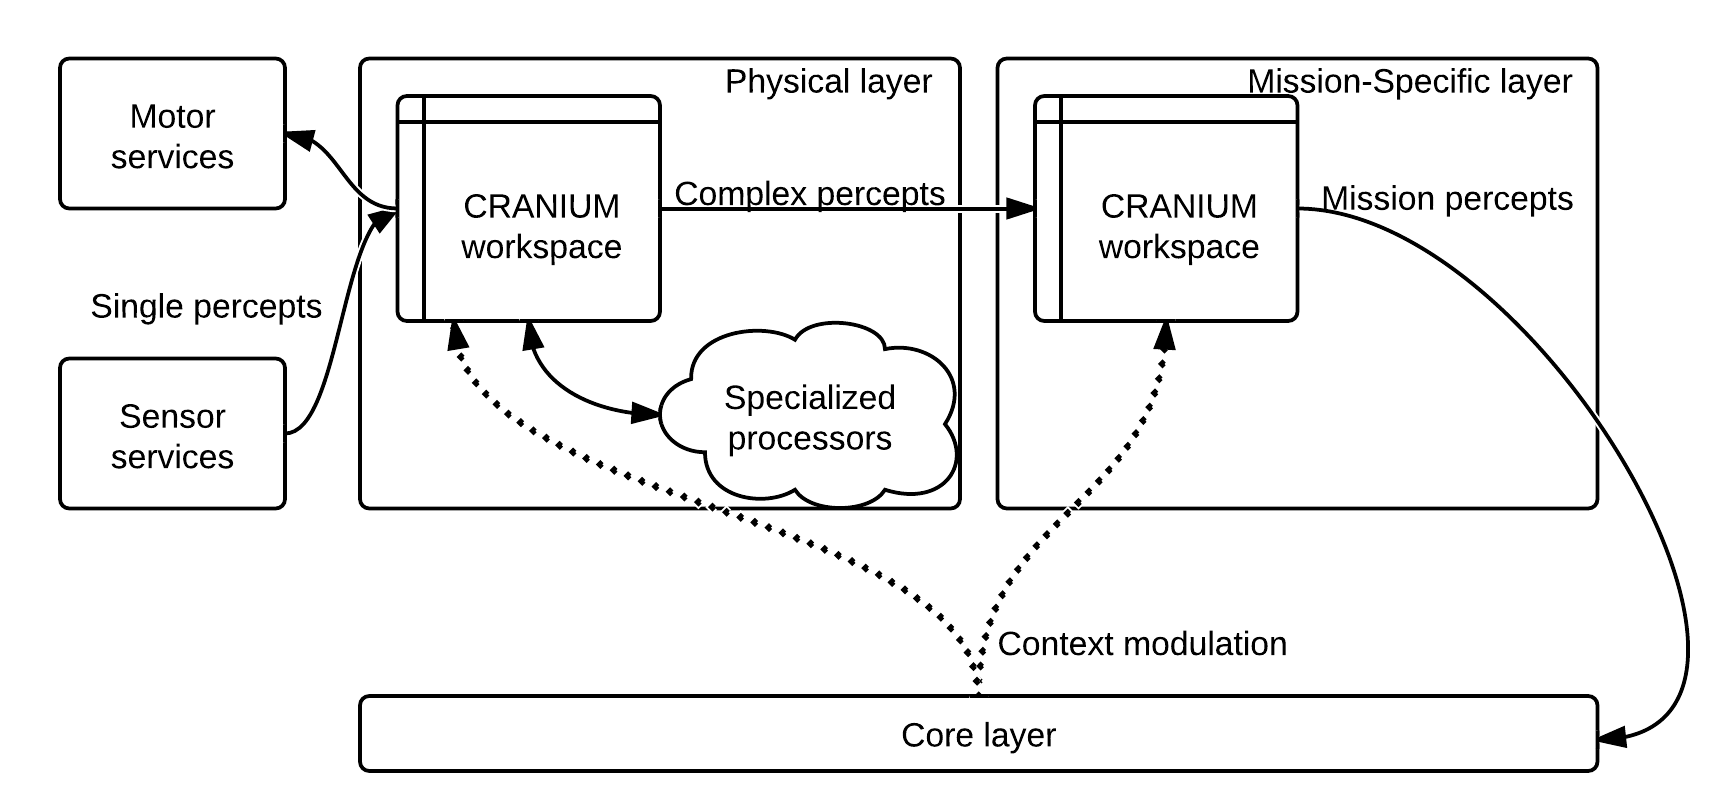
\includegraphics[width=\textwidth]{graphics/ceracranium.png}
\caption{Overview of the CERA-CRANIUM architecture.}
\label{fig:cera-cranium}
\end{figure}
This is a two-fold architecture, as reflected in the name. {\em CRANIUM} is a more generic tool for creation of a high amount of parallel processes operating with shared workspaces. {\em CERA} uses these services for creating a dynamic and adaptable system which operates on perceptions and generates actions, based on a cognitive model.\cite{arrabales2009gamechars} It has been used for making agents that act in several different environments, both virtual environments like the computer game Unreal Tournament, as well as real environments, where it has been embodied in small robots that map out unknown environments. \cite{arrabales2009ceracranium} A high-level overview of the architecture can be seen in Figure \ref{fig:cera-cranium}.

\subsection{Cognitive Models in Game AIs}
There have been several implementations of models of cognition into game-playing agents. Examples of this is CERA-CRANIUM, which was used to implement an agent playing Unreal Tournament \cite{arrabales2009ceracranium}, and SORTS which implemented an agent for the real-time strategy game ORTS using the symbolic, cognitive architecture Soar.\cite{wintermute2007sorts} One of the reasons for using computer games for experiments with regards to high-level artificial intelligence is that the characteristics of computer games lend themselves to this, by eliminating noise and uncertainty, and providing a more or less realistic simulated environment.
